\documentclass{scrreprt}
\usepackage{etex}
\usepackage[ngerman]{babel}
\usepackage[utf8]{inputenc}
\usepackage[T1]{fontenc}
\usepackage{amsmath, amssymb}
\usepackage{graphicx}

\usepackage{pgfplots}
\pgfplotsset{compat=1.11}
\usepgfplotslibrary{external}
\usepackage{pgfplotstable}

\usepackage{booktabs}
\usepackage{multirow}
\usepackage{longtable}
%\usepackage{ulsy}
%\usepackage{pst-all}
\usepackage{picture}
\usepackage[automark]{scrpage2}
\usepackage{caption}
\pagestyle{scrheadings}
\ihead[]{Friedrich Hübner 2897111}
\ohead[]{Fiona Paulus 2909625} 

\author{Friedrich Hübner 2897111\\
Fiona Paulus 2909625}
\title{Computerphysik\\Hausarbeit 3}

\begin{document}
\maketitle
\newpage

\chapter*{Aufgabe 1}
\section*{Aufgabenteil (a)}
Rodrigues-Formel:

\[
P_n(x)= \frac{1}{2^n n!} * \frac{d^n}{dx^n} [(x^2-1)^n]
\]

Daraus ergibt sich für $P_4(x)$:

\[
P_4(x)=\frac{1}{2^4 4!} \frac{d^4}{dx^4}((x^2-1)^4) = \frac{1}{2^4 4!} \frac{d^4}{dx^4} (x^8-4x^6+6x^4-4x^2+1))
\]
\[
 = \frac{1}{384} (1680x ^4-1440x^2+144) = \frac{1}{8} (35x^4-30x^2+3)
\]

\section*{Aufgabenteil (b)}

Rekursionsformel:
\[
(n+1)P_{n+1}(x)=(2n+1)xP_n(x)-nP_{n-1}(x)
\]

Daraus ergibt sich für $P_4(x)$:

\[
4P_4(x) = (3+1)P_{3+1} = 7xP_3(x)-3_{3-1}(x)=7x \frac{5x^3}{3x}-3 \frac{1}{2}(3x^2-1) = \frac{1}{4} (\frac{1}{8}(35x^4-30x^2+3))
\]

\[
\Rightarrow P_4(x) = \frac{1}{8} (35x^4-30x^2+3)
\]

\section*{Aufgabenteil (c)}

Nullstellenberechnung durch Substitution von $x^2 = z$

\[
0=35x^4-30x^2+3
\]

\[
\Rightarrow 0=35z^2-30z+3
\]

\[
\Leftrightarrow 0 = z^2-\frac{30}{35}z+\frac{3}{35} \Leftrightarrow z_{1,2}=-\frac{-\frac{6}{7}}{2}\pm \sqrt{(\frac{3}{7})^2-\frac{3}{35}}=\frac{3}{7}\pm\sqrt{\frac{24}{245}}
\]

Durch Resubstitution:

\[
x_0 = -\sqrt{\frac{3}{7}+\sqrt{\frac{24}{245}}}
\]
\[
x_1 = -\sqrt{\frac{3}{7}-\sqrt{\frac{24}{245}}}
\]
\[
x_2 = +\sqrt{\frac{3}{7}-\sqrt{\frac{24}{245}}}=-x_1\]
\[
x_3 = +\sqrt{\frac{3}{7}+\sqrt{\frac{24}{245}}}
=-x_0\]

Berechnung der Wichtungskoeffizienten:

\[
c_i = \int_{-1}^{1} l_i(x)dx
\]
\\
\[
c_0 = \int_{-1}^{1} \frac{(x-x_1)(x-x_2)(x-x_3)}{(x_0-x_1)(x_0-x_2)(x_0-x_3)}dx
\]

\[
\Rightarrow \int_{-1}^{1} \frac{(x-x_1)(x+x_1)(x+x_0)}{(x_0-x_1)(x_0+x_1)(2x_0)}dx = \int_{-1}^{1}\frac{(x^2-x_1^2)(x+x_0)}{(x_0^2 - x_1^2)2x_0}dx = \frac{1}{(x_0^2-x_1^2)2x_0} (\frac{2}{3}x_0 - 2x_1^2x_0)
\]
\[
=\frac{\frac{1}{3}-x_1^2}{x_0^2 - x_1^2}
=\frac{\frac{1}{3}-\frac{3}{7}+\sqrt{\frac{24}{245}}}{\frac{3}{7}+\sqrt{\frac{24}{245}}-\frac{3}{7}+\sqrt{\frac{24}{245}}} = \frac{18-\sqrt{30}}{36}
\]
\\
\[
c_1 = \int_{-1}^{1} \frac{(x-x_0)(x-x_2)(x-x_3)}{(x_1-x_0)2x_1(x_1+x_0)}dx = \frac{\frac{1}{3}-x_0^2}{x_1^2-x_0^2}=\frac{18+\sqrt{30}}{36}
\]
\\
\[
c_2 = \int_{-1}^{1} \frac{(x+x_3)(x+x_2)(x+x_0)}{(-x_1+x_3)(x_2-x_1)(-x_1+x_0)}dx
\]

Änderung der Variable $x=-t$

\[
= \int_{-1}^{1} \frac{(t-x_3)(t-x_2)(t-x_0)}{(x_1-x_3)(x_1-x_2)(x_1-x_0)}dt = c_1
\]
\\
\[
c_3 = \int_{-1}^{1}\frac{(x+x_3)(x+x_2)(x+x_1)}{(x_3-x_0)(-x_0+x_2)(-x_0+x_1)} dx
\]

Änderung der Variable $x=-t$

\[
= \int_{-1}^{1}\frac{(t-x_3)(t-x_2)(x-x_1)}{(x_0-x_3)(x_1-x_2)(x_0-x_1)}dt = c_0
\]

\section{Aufgabenteil (d)}

Berechnung mithilfe der Legendre-Polynome:

\[
\int_{-1}^{1}e^{-x} \approx \sum_{i=0}^{3} c_i\cdot e^{-x_i}
\]
\[
= \frac{18-\sqrt{30}}{36}*e^{-\sqrt{\frac{3}{7}+\sqrt{\frac{24}{245}}}}
+\frac{18+\sqrt{30}}{36}*e^{-\sqrt{\frac{3}{7}-\sqrt{\frac{24}{245}}}}
+\frac{18+\sqrt{30}}{36}*e^{\sqrt{\frac{3}{7}-\sqrt{\frac{24}{245}}}}
+\frac{18-\sqrt{30}}{36}*e^{\sqrt{\frac{3}{7}+\sqrt{\frac{24}{245}}}}
\]
\[
=2.350402092156377
\]

Berechnung durch direkte Integration:

\[
\int_{-1}^{1} e^{-x}dx = e-\frac{1}{e}=2.3504023872876028
\]

Berechnung des Fehlers:

\[
\Delta = 2.3504023872876028-2.350402092156377 = 2.95\cdot 10^{-7}
\]

Berechnung des Fehlers mithilfe der Legendre Polynome

\[
\Delta = \int_{-1}^{1}f(x)dx - \sum_{i=0}^{n}f(x) = \frac{2^{2n+3}((n+1)!)^4}{((2n+2)!)^3(2n+3)}f^{(2n+2)}(\xi)
\]
\[
=\frac{2^{2*3+3}((3+1)!)^4}{((2*3+2)!)^3(2*3+3)}\frac{d^8}{dx^8}e^{-\xi}
\]

Für $\xi \in [-1,1] \Rightarrow \xi=-1$ eingesetzt:
\[
=\frac{2^9 4!^4}{8!^3 9} e = 7.8271802*10^{-7}
\]

\chapter*{Aufgabe 2}
\section*{allgemeine Hinweise}
Das Programm zur Aufgabe 2 wurde unter Linux Mint mit "g++ -std=c++11 -g -Wall -Wextra -pedantic-errors pendelschwingdauer.cpp -o pendelschwingdauer.exe" kompiliert.

\section*{Lösung}
Zur bestimmung der Abweichung der Schwingungsdauer T vom harmonischen Wert als Funktion von $\phi_0$ wird mit dem Newton-Cotes-Verfahren numerisch integriert ("pendelschwingdauer.cpp").
Dazu werden die Simpson-Koeffizienten verwendet und in die Newton-Cotes-Formel eingesetzt. 
\[
\int_{a}^{b}f(x)dx \approx \frac{(a-b)}{n} \sum_{i=0}^{n} \omega_i f(x_i) 
\]
Wobei $\omega_i$ die Simpson Koeffizienten sind und die $x_i$ die zugehörigen Stützstellen. Diese Rechnung wird für $\phi_0$ zwischen $0^\circ$ und $180^\circ$ wiederholt und in ihr Ergebnis in der Datei "data2.txt" gespeichert.\\
Das Ergebnis wird mit der Datei "2.plt" geplottet.
\begin{center}
	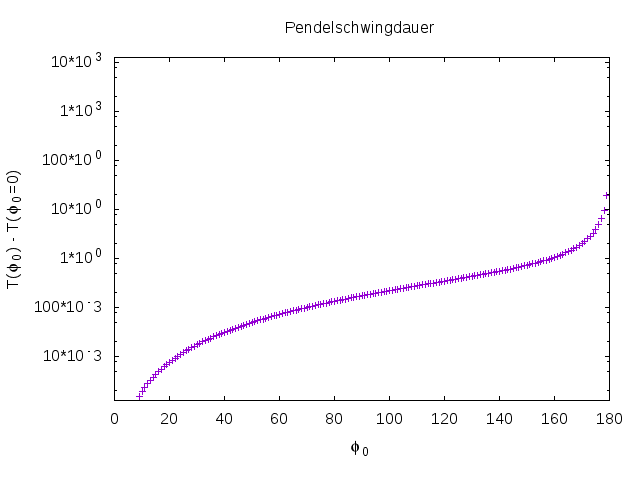
\includegraphics[scale=0.6]{2.png}
	\captionof{figure}{Abweichung der Pendelschwingdauer T/s vom harmonischen Wert in Abhängigkeit der Auslenkung $\phi_0/^\circ$}
\end{center}

\section*{Sonstige Abgegebene Dateien}
\subsection*{2.plt}
Die Plot-Datei für den Plots in der Abgabe.
\subsection*{data2.txt}
Ausgabedatei des Programms "pendelschwingdauer.cpp".

\chapter*{Aufgabe 3}
\section*{allgemeine Hinweise}
Das Programm zur Aufgabe 3 wurde unter Linux Mint mit "g++ -std=c++11 -g -Wall -Wextra -pedantic-errors planckkurve.cpp -o planckkurve.exe" kompiliert.

\section*{Aufgabenteil (a)}
Es wurde die Planckkurve $S(\lambda)$ geplottet für die Temperaturen $T=100K$, $T=500K$ und $T=1000K$.("3a.plt", "3a-.plt").
\begin{center}
	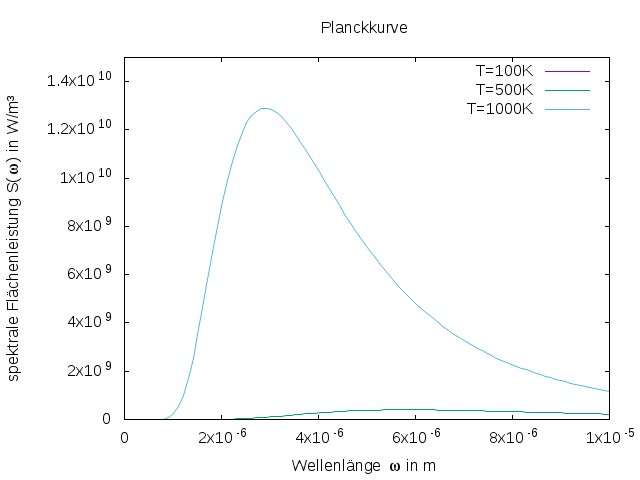
\includegraphics[scale=0.6]{3a_1000.jpeg}
	\captionof{figure}{Planckkurven}
\end{center}
\begin{center}	
	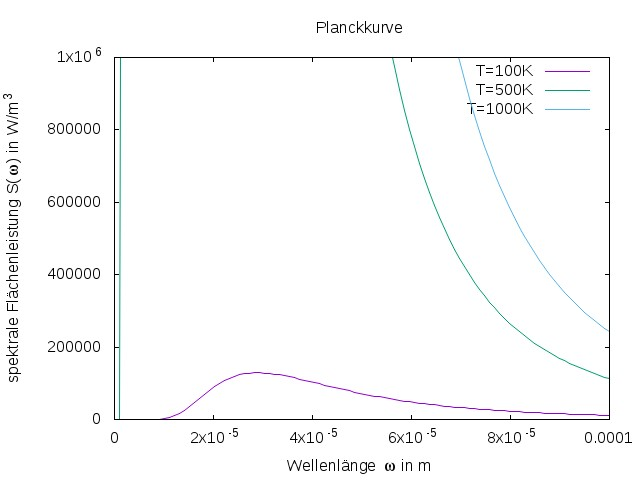
\includegraphics[scale=0.6]{3a_100.jpeg}
	\captionof{figure}{Planckkurve Ausschnitt}
\end{center}

\section*{Aufgabenteil (b)}
Um den Energieanteil des sichtbaren Lichts als Funktion der Temperatur zu bestimmen, wird über die Energieverteilung $S(\lambda)$ numerisch ("planckkurve.cpp") mit dem Newton-Cotes-Verfahren integriert. Hierzu werden die Milne-Koeffizienten als $\omega_i$ in die obige Newton-Cotes-Formel eingesetzt.

\[
E(T)=\frac{\int_{380*10^{-9}}^{780*10^{-9}}S(\lambda)d\lambda}{\int_{0}^{\infty}S(\lambda)d\lambda} = \frac{1}{\frac{dP}{dA}} \int_{380*10^{-9}}^{780*10^{-9}}S(\lambda)d\lambda
\]

Dies wird für Temperaturen zwischen 100K und 50000K in 200K Schritten wiederholt und die daraus errechneten Werte werden in "data3.txt" gespeichert. Diese Werte werden mit "3b.plt" geplottet.

\begin{center}
	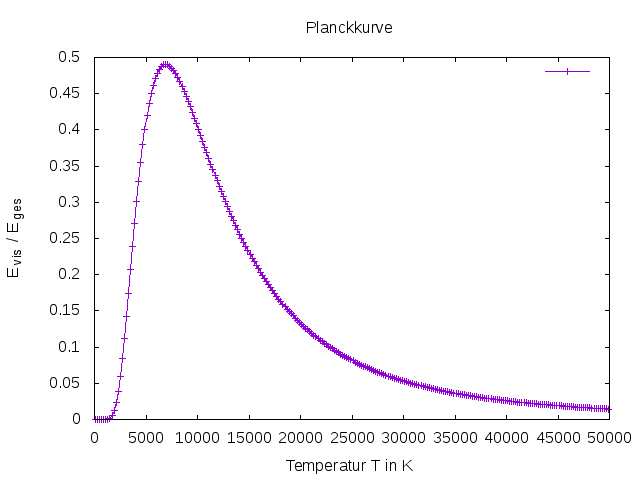
\includegraphics[scale=0.6]{3b.png}
	\captionof{figure}{Energieanteil des sichtbaren Lichts als Funktion der Temperatur}
\end{center}

\section*{Sonstige Abgegebene Dateien}
\subsection*{3a.plt, 3a-.plt, 3b.plt}
Die Plotdateien zur Erzeugung der Planckfunktionen und der Funktion zur Abhängigkeit des Energieanteils des sichtbaren Bereichs in Abhängigkeit der Temperatur.
\subsection*{data3.txt}
Ausgabedatei des Programms "planckkkurve.cpp".

\chapter*{Aufgabe 4}
\section*{Allgemeine Hinweise}
Das Programm wurde unter Windows 10 mit "g++ -o abgabe3\_4.exe -Wall -Wextra -std=c++0x -O2 -static abgabe3\_4.cpp"\;kompiliert.\\
Das Programm wird gestartet mit 'abgabe3\_4 $H_0\;\Omega_{\Lambda}\;\Omega_{m}\;\Omega_{r}$', wobei $H_0$ in km/s/Mpc ist. 

\section*{Idee}
Da die eine Integralgrenze $\infty$ ist, kann man die Funktion nicht mit den normalen Methoden integrieren. Deswegen wird zuerst eine Substution $a = \frac{1}{1+z}$ durchgeführt.
\begin{align}
t(z) &= \frac{1}{H_0} \int\limits_z^\infty \cfrac{dz'}{(1+z')\sqrt{E(\frac{1}{1+z})}}\\
     &= \frac{1}{H_0} \int\limits_\frac{1}{1+z}^0 \cfrac{a'}{\sqrt{E(a')}} -\frac{1}{a'^2} da'\\
     &= \frac{1}{H_0} \int\limits_0^a \cfrac{1}{a'\sqrt{E(a')}} da'\\
     &= \frac{1}{H_0} \int\limits_0^a f(a') da'
\end{align}
Da heute z = 0 ist, liegt $z \in [0,\infty)$. Somit liegt $a \in [0,1)$. Dieses Integral kann nun mit einer der bekannten Methoden berechnet werden.\\

Da die zu integrierende Funktion bei a'=0 nicht definiert ist, muss man noch den Grenzwert für $a' \to 0$ berechnen:\\
$\lim\limits_{a'\to 0} a'^2 E(a') = \lim\limits_{a'\to 0} a'^2 \Omega_\Lambda + \Omega_m/a' + \Omega_r/a'^2 + \Omega_k = \infty$ für $\Omega_m \neq 0, \Omega_r \neq 0$, sonst $\Omega_k$.\\
Damit gilt für $\lim\limits_{a'\to 0} f(a') = 0$ für $\Omega_m \neq 0, \Omega_r \neq 0$, sonst $1/\sqrt{\Omega_k}$.\\ 

\section*{Programm}
Das Integral wurde mit der (zusammengesetzten) Trapezformel berechnet. Man kann das Ergebnis t(a) wiederverwenden, um $t(a+\Delta a) = t(a) + \frac{1}{H_0} \int\limits_a^{a+\Delta a} f(a') da'$ zu berechnen. Im Programm selber wird zuerst nur die Stammfunktion von f numerisch bestimmt und in einem Array gespeichert. Zur Ausgabe wird linear zwischen den zwei nächsten ermittelten Werten interpoliert und dieser Wert durch $H_0$ geteilt.

\section*{Beispiele}
Hier sind die in Aufgabe b) und c) geforderten Diagramme. Beide Kurven wurden in ein Diagramm gezeichnet, das einmal normal und einmal logarithmisch dargestellt wurde.
\begin{center}
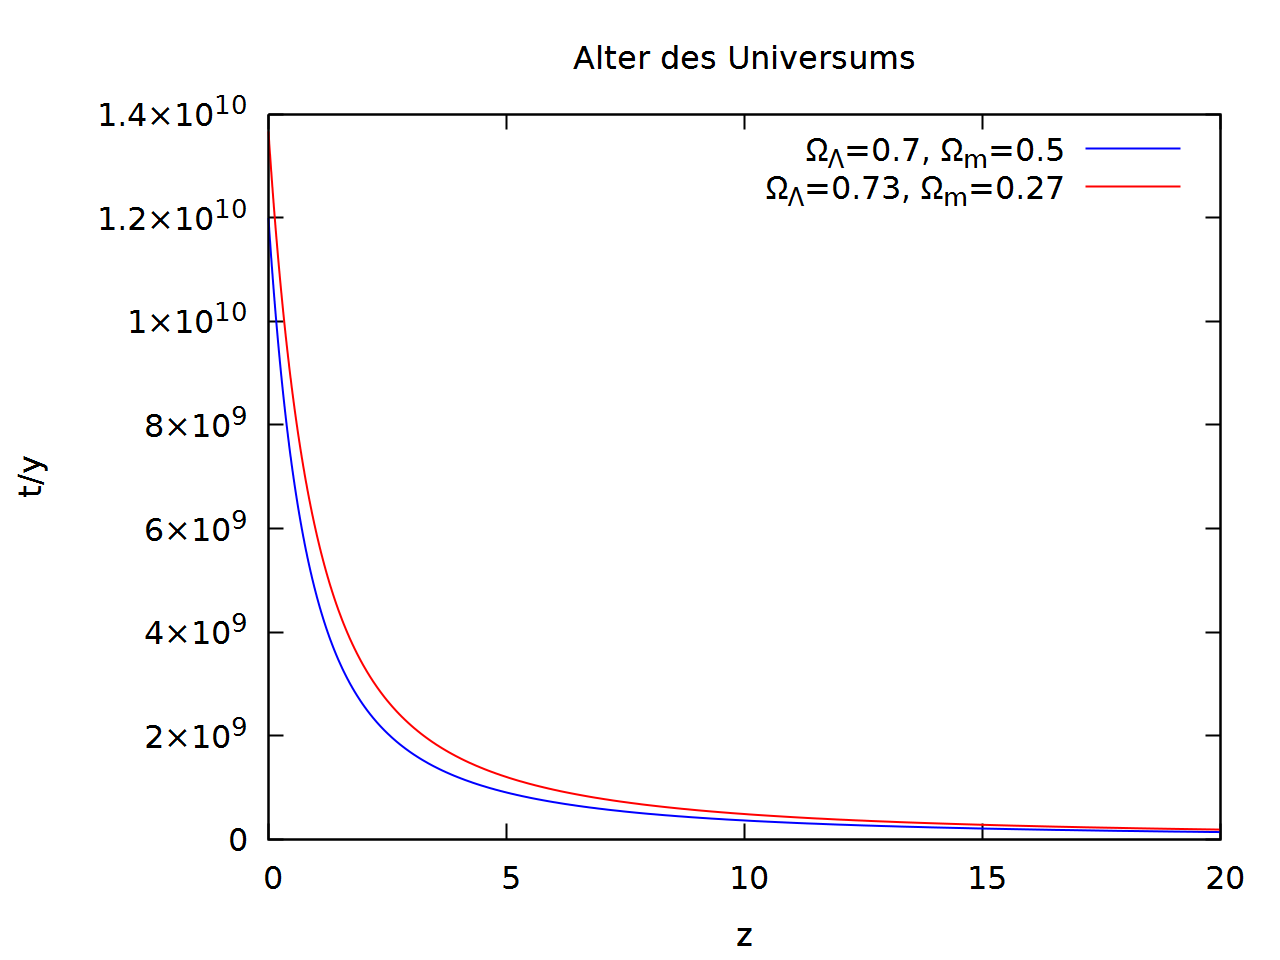
\includegraphics[scale=0.3]{4_plot_final} 
\captionof{figure}{Normaler Plot}
\end{center}
\begin{center}
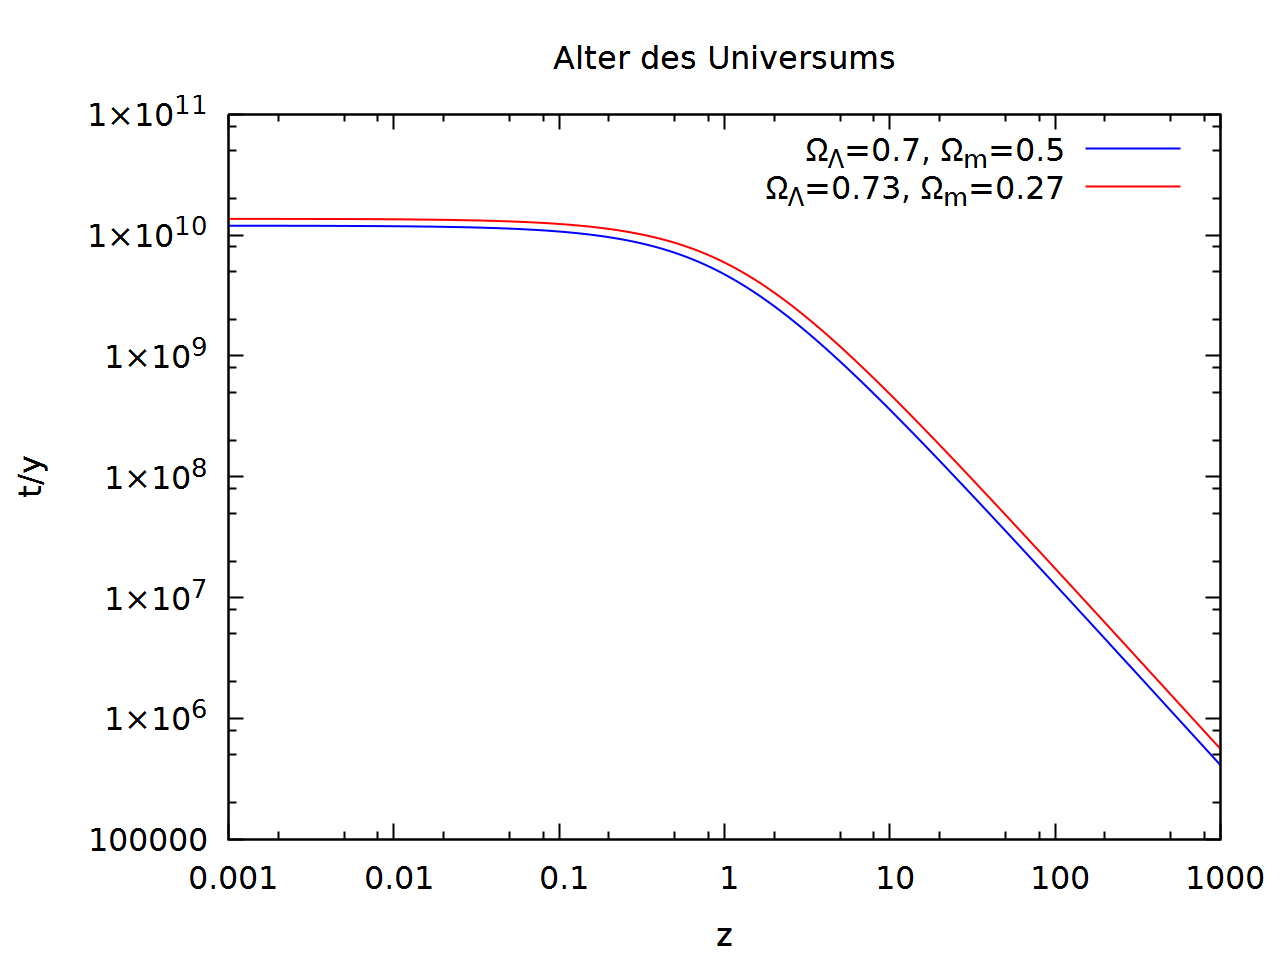
\includegraphics[scale=0.3]{4_plot_log_final} 
\captionof{figure}{Logarithmischer Plot}
\end{center}

\section*{Sonstige abgegebene Dateien}
\subsection*{plot\_final.plt}
Die Plot-Datei für die beiden Plots in der Abgabe.
\subsection*{b.txt}
Enthält die Plotdaten für b)
\subsection*{c.txt}
Enthält die Plotdaten für c)

\chapter*{Aufgabe 5}
\section*{Allgemeine Hinweise}
Zu a):\\
Das Programm wurde unter Windows 10 mit "g++ -o abgabe3\_5\_bessel.exe -Wall -Wextra -std=c++0x -O2 -static abgabe3\_5\_bessel.cpp"\;kompiliert.\\
Das Programm wird gestartet mit 'abgabe3\_5\_bessel n l r', wobei $n \in \mathbb{N}$ der Parameter der Besselfunktion ist und $l,r$ das Intervall, auf dem die Besselfunktion berechnet werden soll.\\

Zu b):\\
Das Programm wurde unter Windows 10 mit "g++ -o abgabe3\_5.exe -Wall -Wextra -std=c++0x -O2 -static abgabe3\_5.cpp"\;kompiliert.\\
Das Programm wird gestartet mit 'abgabe3\_5'. 

\section*{a) (abgabe3\_5\_bessel.cpp)}
Der Funktionswert der Besselfunktion wird mithilfe der zusammengesetzten Trapezformel berechnet. Im Intervall (l,r) wird an 1000 gleichverteilten x-Werten der Funktionswert berechnet und ausgegeben.

\begin{center}
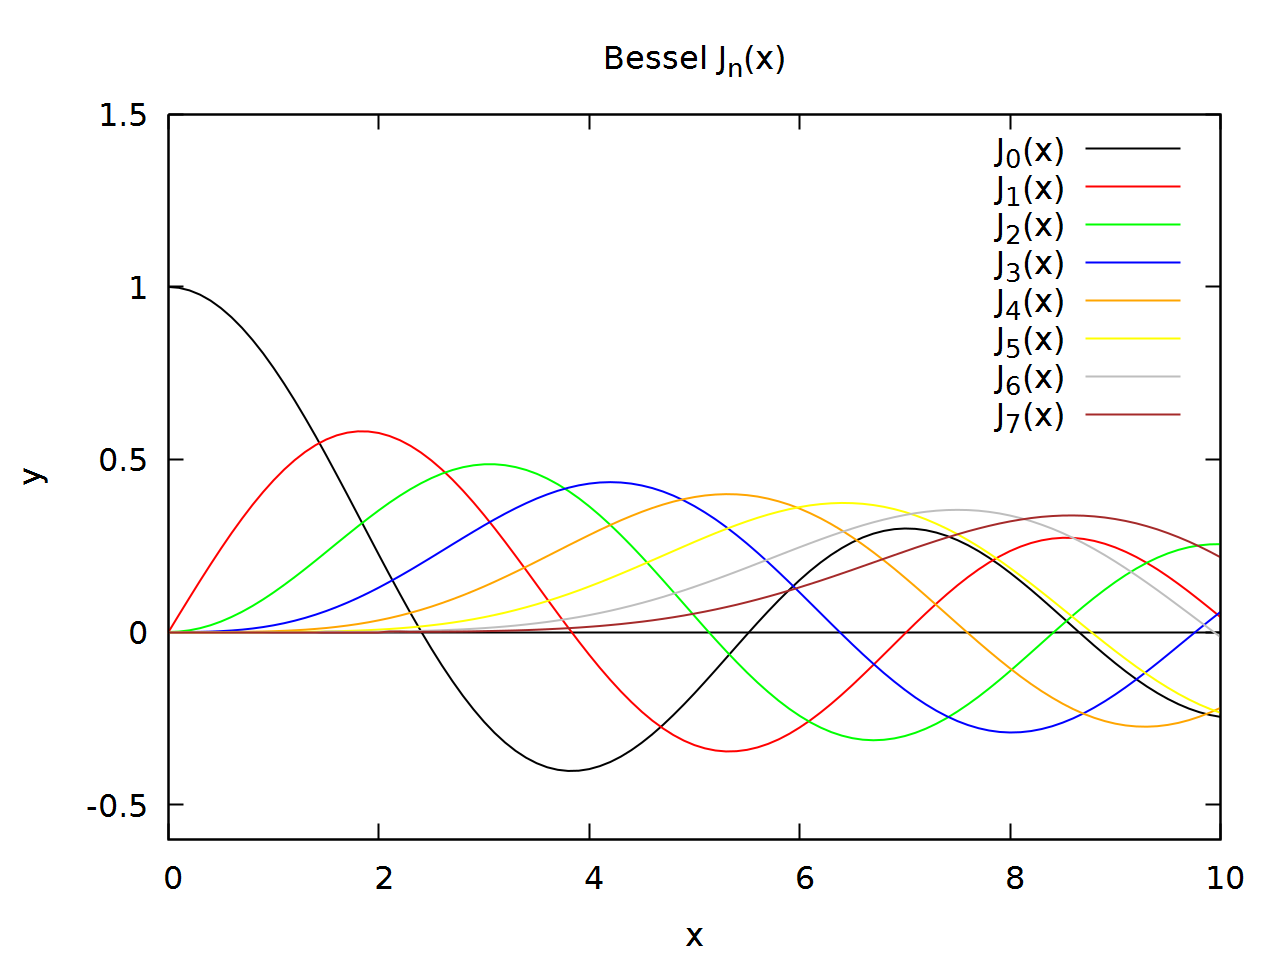
\includegraphics[scale=0.3]{5_plot_bessel.png}
\captionof{figure}{Die ersten 8 Besselfunktionen}
\end{center}

\section*{b) (abgabe3\_5.cpp)}
Zur Berechnung der Besselfunktion wird der Algorithmus aus a) verwendet.\\
Es wird einfach die Formel in der Aufgabenstellung bei mehreren äquidistanten $\theta$ ausgewertet. Die Ausgabe erfolgt in slit.txt\\

Dabei ergibt sich folgendes Bild:\\
\begin{center}
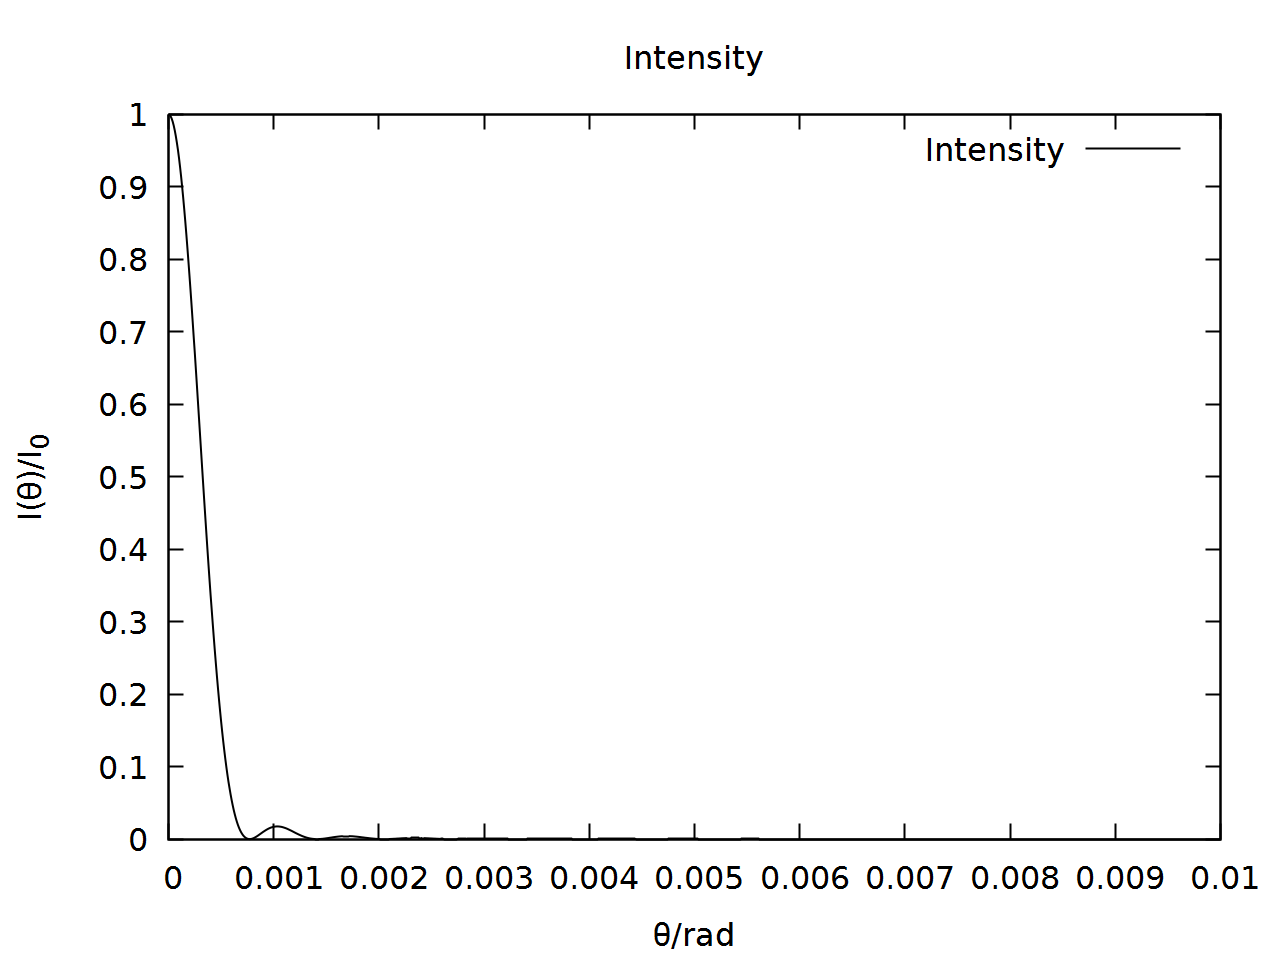
\includegraphics[scale=0.3]{5_plot_slit.png}
\captionof{figure}{Beugungsbild an einer Kreisblende}
\end{center}
\begin{center}
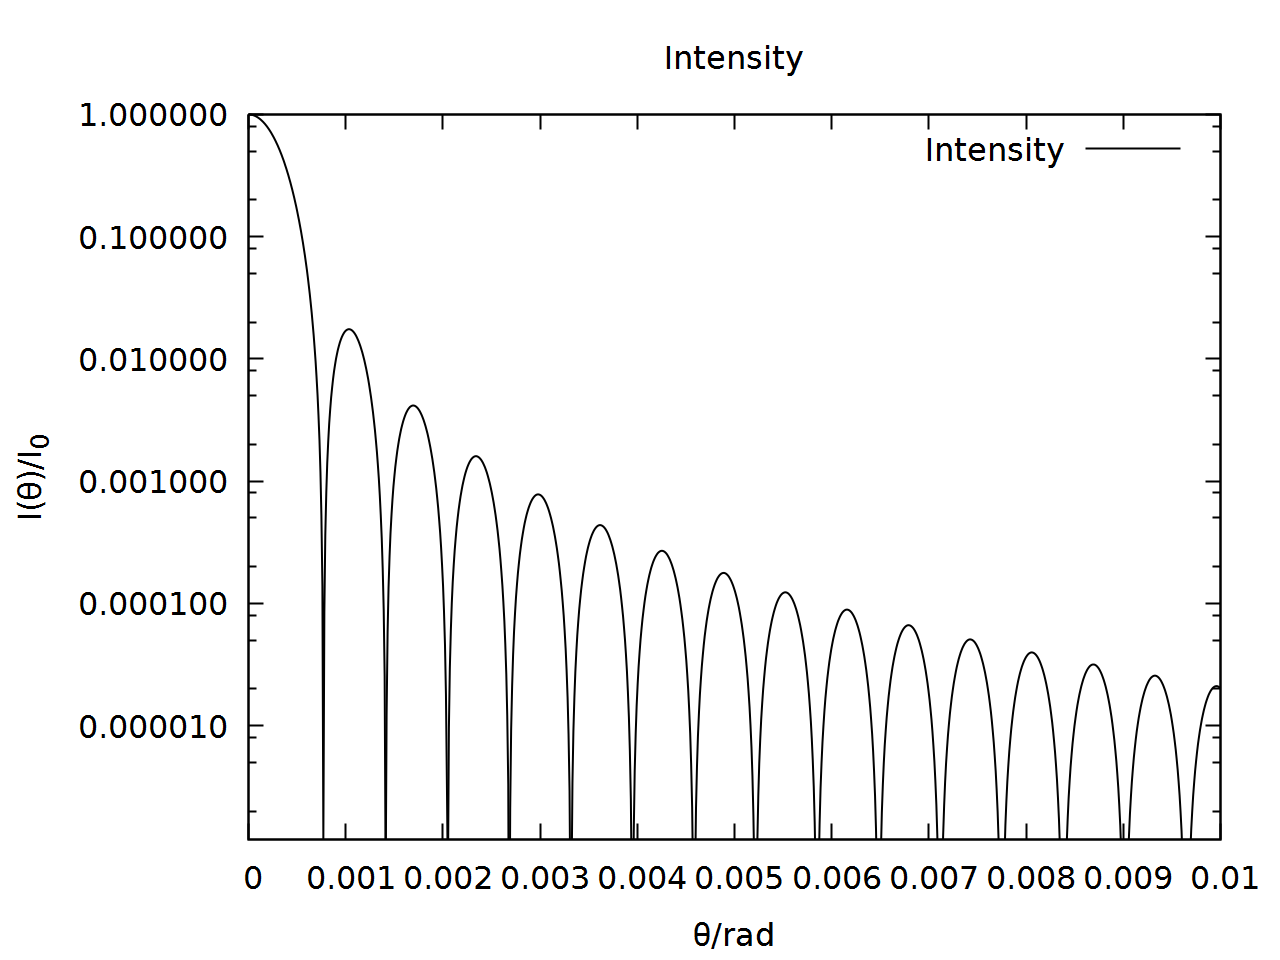
\includegraphics[scale=0.3]{5_plot_slit_log.png}
\captionof{figure}{Beugungsbild an einer Kreisblende (logarithmisch)}
\end{center}

\section*{c) (abgabe3\_5.cpp)}
Im selben Programm werden auch noch Maxima und Minima bestimmt. Dazu werden alle Werte durchgegangen. Ist ein Wert sowohl größer als der Vorgänger als auch der Nachfolger, so ist an dieser Stelle ein Maxmimum. Für Minima ist es analog. Man speichert sich zunächst nur den Index des Punktes, an dem die Extremstelle vorliegt und berechnet später daraus den Winkel.\\
Dabei ergeben sich folgende Maxima und Minima:\\
\begin{center}
\captionof{table}{Maxima}
\begin{tabular}{ccc}
\toprule
n & $\theta/rad$ & $I(\theta)/I_0$\\
\midrule
0 & 0 & 1\\
1 & 0.00103103 & 0.0174927\\
2 & 0.00169169 & 0.00415657\\
3 & 0.00234234 & 0.0016005\\
4 & 0.00298298 & 0.000779314\\
5 & 0.00361361 & 0.000436851\\
6 & 0.00425425 & 0.000269287\\
7 & 0.00488488 & 0.000177494\\
8 & 0.00552553 & 0.00012319\\
9 & 0.00615616 & 8.89594e-005\\
10 & 0.00678679 & 6.6293e-005\\
\bottomrule
\end{tabular}
\end{center}

\begin{center}
\captionof{table}{Minima}
\begin{tabular}{ccc}
\toprule
n & $\theta/rad$\\
\midrule
1 & 0.000770771\\
2 & 0.00141141\\
3 & 0.00205205\\
4 & 0.00268268\\
5 & 0.00331331\\
6 & 0.00395395\\
7 & 0.00458458\\
8 & 0.00521522\\
9 & 0.00584585\\
10 & 0.00648649\\
\bottomrule
\end{tabular}
\end{center}

\section*{Sonstige abgegebene Dateien}
\subsection*{plot\_bessel.plt}
Die Plot-Datei für die Besselfunktionen
\subsection*{plot\_slit.plt}
Die Plot-Datei für die Kreisblende
\subsection*{slit.txt}
Enthält die Plotdaten für die b)
\end{document}